% ─────────────────────────────────────────────────────────────────────────────
% Captions for the fixed-effect (coefficient) figures produced by
% plot_fixef() in GLMM_analysis.ipynb.  Figures are the *_no_title.pdf files:
% the axis carries the symbol, the wording lives here.
%
% Curriculum direction is contrast-coded, forward = +0.5 and reverse = -0.5, so
% each model is fitted once: the D coefficient is the forward-minus-reverse
% difference and the t coefficient is the average slope over both directions.
% Every model is a linear mixed model on the change score
% \(\Delta = \mathrm{acc} - \mathrm{acc}_{\text{base}}\), fitted with lme4/lmerTest;
% points are estimates, bars 95\% CIs, and red marks a CI excluding zero.
% ─────────────────────────────────────────────────────────────────────────────


% ══════════════ 1. curriculum · inference ══════════════

\begin{figure}[t]
\centering
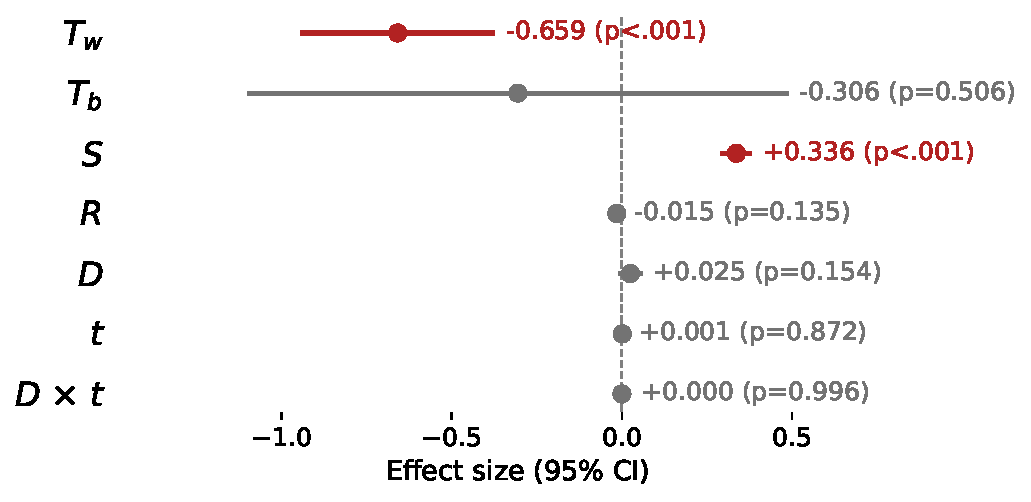
\includegraphics[width=\linewidth]{figures/fixef_curriculum_inference_no_title.pdf}
\caption{\textbf{What drives the change in inference accuracy on the curriculum
tasks.} Fixed-effect estimates (points) with 95\% confidence intervals (bars)
from a linear mixed model on the change score
\(\Delta=\mathrm{acc}-\mathrm{acc}_{\text{base}}\); red marks an interval that
excludes zero. Predictors are
\(T_{w}\), the within-task baseline (a model's baseline accuracy on that task
minus its own mean across tasks, \(\bar{T}_{m,t}-\bar{T}_{m}\));
\(T_{b}\), the between-model baseline (a model's mean baseline accuracy minus the
grand mean, \(\bar{T}_{m}-\bar{T}\));
\(S\), a trained-session indicator that turns on once the task has been trained;
\(R\), how long ago that training happened;
\(D\), the curriculum direction, contrast-coded as \(+0.5\) for forward and
\(-0.5\) for reverse, so its coefficient is the forward-minus-reverse difference;
\(t\), centred training time in sessions, whose coefficient is the average slope
over both directions; and their interaction \(D\times t\), which tests whether
the two curricula improve at different rates.
Random intercepts are fitted for model, task, and their interaction
(\(1|\text{model}\), \(1|\text{task}\), \(1|\text{model}{:}\text{task}\)).}
\label{fig:fixef_curriculum_inference}
\end{figure}


% ══════════════ 2. curriculum · probing ══════════════

\begin{figure}[t]
\centering
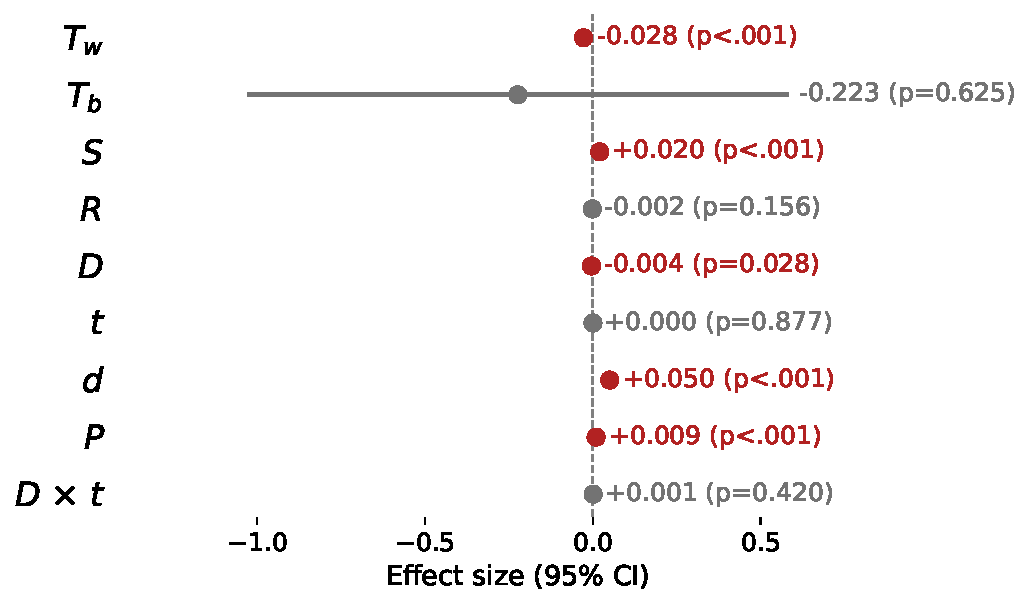
\includegraphics[width=\linewidth]{figures/fixef_curriculum_probing_no_title.pdf}
\caption{\textbf{What drives the change in linear-probe accuracy on the
curriculum tasks.} Fixed effects with 95\% CIs from a linear mixed model on
\(\Delta=\mathrm{acc}-\mathrm{acc}_{\text{base}}\); red marks a CI excluding zero.
Predictors are \(T_{w}\) (within-task baseline, \(\bar{T}_{m,t}-\bar{T}_{m}\)),
\(T_{b}\) (between-model baseline, \(\bar{T}_{m}-\bar{T}\)),
\(S\) (trained-session indicator), \(R\) (recency of that training),
\(D\) (curriculum direction, contrast-coded \(+0.5\) forward / \(-0.5\) reverse),
\(t\) (centred training time; the coefficient is the average slope over both
directions), \(d\) (relative representation depth, \(0=\)~first layer,
\(1=\)~last layer), \(P\) (projector-layer indicator, fitted off the depth axis),
and the interaction \(D\times t\). Depth enters linearly: the quadratic term was
not significant and the linear form had the lower AIC. Random intercepts: model,
task, model\(\times\)task, and probe cell.}
\label{fig:fixef_curriculum_probing}
\end{figure}


% ══════════════ 3. curriculum · probing · direction × depth ══════════════

\begin{figure}[t]
\centering
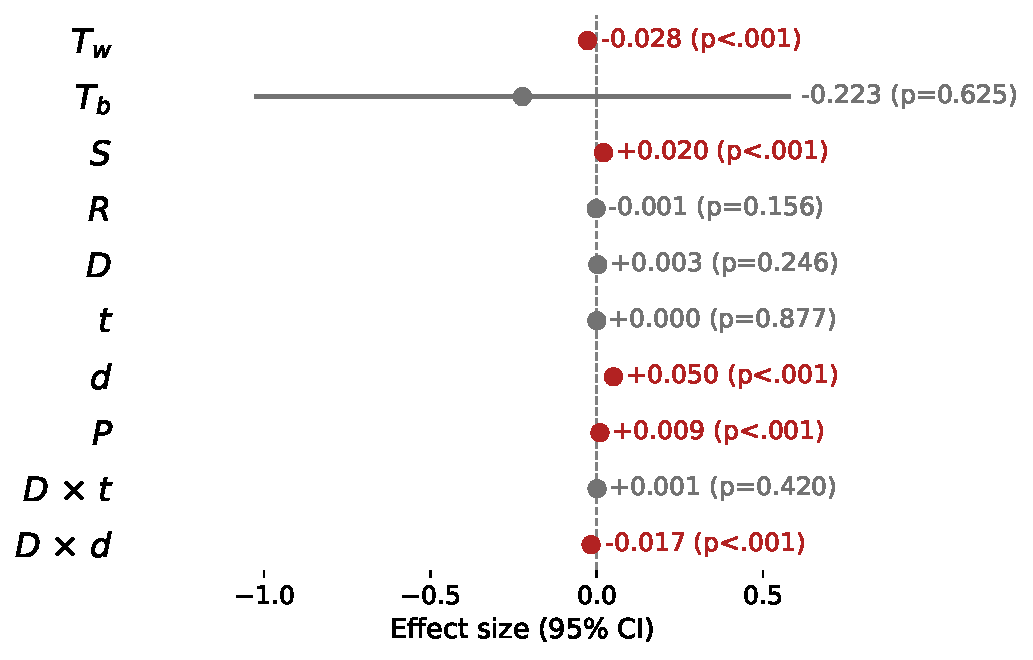
\includegraphics[width=\linewidth]{figures/fixef_curriculum_probing_depth_no_title.pdf}
\caption{\textbf{Does the curriculum direction change \emph{where} in the network
the representation moves?} The model of
Fig.~\ref{fig:fixef_curriculum_probing} extended with a direction-by-depth
interaction: a non-zero \(D\times d\) means the depth profile of the probe gain
differs between the two curricula. Predictors are \(T_{w}\), \(T_{b}\)
(baseline terms), \(S\) (trained-session indicator), \(R\) (recency),
\(D\) (curriculum direction, \(+0.5\) forward / \(-0.5\) reverse), \(t\) (centred
training time), \(d\) (relative representation depth, 0--1), \(P\) (projector
indicator), and the interactions \(D\times t\) and \(D\times d\). Random
intercepts: model, task, model\(\times\)task, probe cell. Bars are 95\% CIs; red
marks a CI excluding zero. This analysis is exploratory.}
\label{fig:fixef_curriculum_probing_depth}
\end{figure}


% ══════════════ 4. transfer benchmarks · inference ══════════════

\begin{figure}[t]
\centering
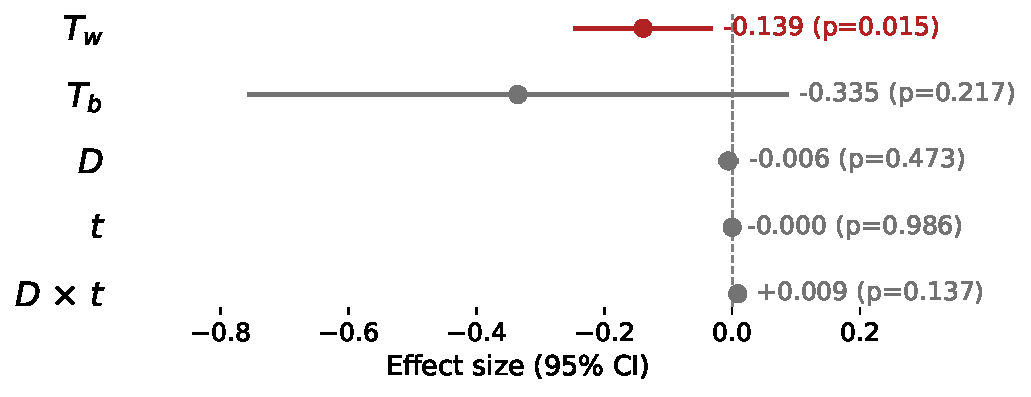
\includegraphics[width=\linewidth]{figures/fixef_benchmark_inference_no_title.pdf}
\caption{\textbf{Transfer to the held-out benchmarks: inference accuracy.} The
benchmarks are never trained on, so the model carries no trained-session or
recency term and the whole training exposure is summarised by \(t\); the test of
interest is \(D\times t\), i.e.\ whether the two curricula transfer at different
rates. Predictors are \(T_{w}\) (within-task baseline,
\(\bar{T}_{m,t}-\bar{T}_{m}\)), \(T_{b}\) (between-model baseline,
\(\bar{T}_{m}-\bar{T}\)), \(D\) (curriculum direction, contrast-coded \(+0.5\)
forward / \(-0.5\) reverse), \(t\) (centred training time in sessions, averaged
over both directions), and \(D\times t\). Random intercepts: model, task,
model\(\times\)task. Points are estimates, bars 95\% CIs; red marks a CI
excluding zero. Baseline accuracies of the untrained models are given in
Table~\ref{tab:benchmark_base}.}
\label{fig:fixef_benchmark_inference}
\end{figure}


% ══════════════ 5. transfer benchmarks · probing ══════════════

\begin{figure}[t]
\centering
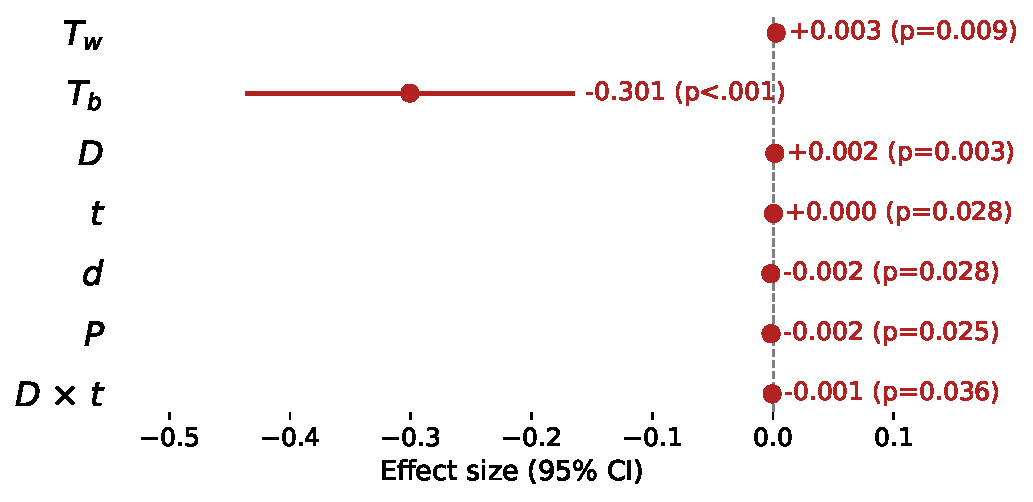
\includegraphics[width=\linewidth]{figures/fixef_benchmark_probing_no_title.pdf}
\caption{\textbf{Transfer to the held-out benchmarks: linear-probe accuracy.}
As in Fig.~\ref{fig:fixef_benchmark_inference}, but with probe accuracy as the
response and representation depth added, so the model asks both whether transfer
differs by curriculum direction (\(D\times t\)) and whether it is concentrated at
a particular depth. Predictors are \(T_{w}\) (within-task baseline), \(T_{b}\)
(between-model baseline), \(D\) (curriculum direction, \(+0.5\) forward /
\(-0.5\) reverse), \(t\) (centred training time), \(d\) (relative representation
depth, \(0=\)~first layer, \(1=\)~last layer), \(P\) (projector-layer indicator),
and \(D\times t\). Random intercepts: model, task, model\(\times\)task, probe
cell. Bars are 95\% CIs; red marks a CI excluding zero.}
\label{fig:fixef_benchmark_probing}
\end{figure}
